\section{Evaluation}

\begin{figure}
\centering
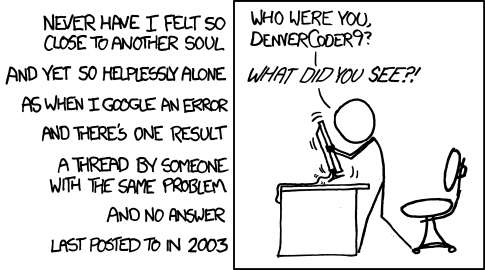
\includegraphics[width=\linewidth]{wisdom_of_the_ancients}
\caption{A sample black and white graphic
that is inline}
\end{figure}

\begin{figure*}
\centering
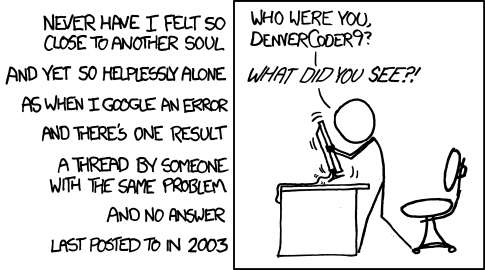
\includegraphics[height=50ex]{wisdom_of_the_ancients}
\caption{A sample black and white graphic
that needs to span two columns of text.}
\end{figure*}

In this section, we report on our evaluation of the practicality of
our discipline. 

\subsection{Quantitative Evaluation}

{\bf RQ1.} Under the assumption of an idealized API test suite, does
our tool detect SemVer violations?

\subsection{User Study Evaluation}
Our second evaluation is a user study of the efficacy of our
approach. We focus on 

{\bf RQ2.} Without any assumptions about the test suite, does our tool
detect SemVer violations?

{\bf RQ3.} How difficult is it to adopt our discipline of writing API
tests?

To answer {\bf RQ2}, we manually inspected the {\em possible} SemVer
violations reported by our tool, in order to determine whether any of
them represent true violations. In particular, we ask whether the test
failure was due to an illegal change in the interface (in which case
the failure is a true violation), due to non-adherence to our
discipline, or for some other reason.

While reviewing the violations for {\bf RQ2}, we refactored failing
tests to adhere to our discipline whenever possible. To answer {\bf
  RQ3}, we recorded the time required for the refactoring. We also
looked for any inherent limitations of our approach that may make
adherence more difficult.

This study was conducted by the authors, who had no prior knowledge of
the internals of Mocha. Lacking ground truth for what the ``true''
interface is, we consulted the Mocha documentation, source code and
comments, and version history to make the best determination
possible. Whenever multiple interpretations were possible, we gave
Mocha developers the benefit of the doubt, choosing the interpretation
that would minimize SemVer violations.

\subsection{Other stuff we learned}
\begin{itemize}
\item A library should upper-bound their dependencies to stay within
  the current major version, since updrading to the next major version
  of a dependency may introduce a breaking change, which in turn could
  cause a breaking change for the library itself. We found this
  problem with mocha, and had to modify its {\tt package.json} file to
  correct it.
\item NPM packages specify a set of {\tt devDependencies} in the {\tt
    package.json}, which are the dependencies needed by the test suite
  but not the library itself. When cross-version testing, it is
  important to use the {\tt devDependencies} of the tests, not those
  of the library. Therefore, we found that we had to modify {\tt
    package.json} of the library each time we ran a cross-version
  test.
\end{itemize}